\documentclass{beamer}

\usepackage[utf8]{inputenc}

\author{Jacob Thomas Errington}
\title{
    git\\
    the stupid content tracker
}
\institute{McGill University}
\date{22 March 2017}

\usepackage{listings}
\usepackage{amsmath,amssymb,amsthm}
\usepackage{tikz}
\usepackage{hyperref}

%%%%% LISTINGS

\lstset{basicstyle=\ttfamily}

%%%%% TIKZ

\usetikzlibrary{arrows,shapes,graphs,calc}

\tikzstyle{every picture}+=[remember picture]
\tikzset{
    ampersand replacement=\&,
    >=stealth',
    shorten >=1pt,
    commit/.style={
        draw=black,
        circle,
        minimum size=3em,
    },
    rootcommit/.style={
        label=below:{root commit},
    },
    branch/.style={},
    branch'/.style={
        draw=blue,
    },
}

%%%%% FONTS

\everymath{\displaystyle}
\usefonttheme{serif}

%%%%% MISC

\newcommand{\HEAD}{\texttt{HEAD}}
\newcommand{\protip}[1]{(\textbf{Protip:} #1)}

\begin{document}

\frame{\titlepage}

\begin{frame}
    \frametitle{Structure of this talk}

    \begin{itemize}
        \item
            Basic concepts in git, from the ground up.

        \item
            Major git commands, and scenarios for using them.

        \item
            GitHub.
    \end{itemize}
\end{frame}

\begin{frame}
    \frametitle{Slides are available online}

    \url{https://files.jerrington.me/git-workshop-2017.pdf}
\end{frame}

\begin{frame}
    \frametitle{Pros and cons of git}

    \begin{description}
        \item[Pros]
            \begin{enumerate}
                \item Decentralized.
                    % No reliance on a central server.
                    % If a central server goes down, it is still possible to
                    % work locally, and even to share your work with others
                    % directly.
                \item Fast.
                \item Popular.
            \end{enumerate}

        \item[Cons]
            \begin{enumerate}
                \item Leaky abstractions.
                \item Arcane command-line syntax.
            \end{enumerate}
    \end{description}
    %
    % Hopefully this talk will make the cons irrelevant:
    % - By explaining how git works at its core, the leakiness of the
    %   abstractions won't be a problem so much as a minor annoyance.
    % - By showing you the commands, especially some of the more exotic ones,
    %   you won't be afraid of running them!
    %
    % You won't be a git expert after one workshop, but hopefully you'll know
    % what's possible and what some of the terminology is.
\end{frame}

\begin{frame}
    \frametitle{Concept: the repository}

    \begin{itemize}
        \item
            A \emph{commit} is a snapshot of the state of your project together
            with pointers to its \emph{parent commits}.

        \item
            A \emph{branch} is a (named) pointer to a commit.
    \end{itemize}

    A repository can be visualized as a diagram
    (formally a \emph{directed acylic graph}).

    \begin{center}
        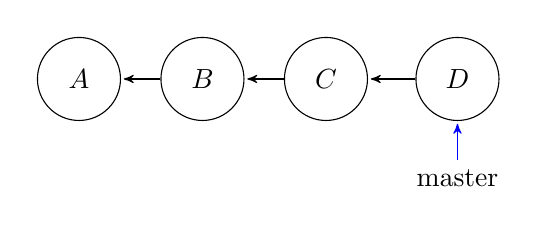
\begin{tikzpicture}
            \matrix[row sep=5mm, column sep=5mm]{
                \node[commit] (A) {$A$} ; \&
                \node[commit] (B) {$B$} ; \&
                \node[commit] (C) {$C$} ; \&
                \node[commit] (D) {$D$} ; \\
                \& \& \& \node[branch] (master) {master} ; \\
            } ;

            \graph[use existing nodes]{
                master ->[branch']
                D -> C -> B -> A ;
            } ;
        \end{tikzpicture}
    \end{center}

    In this case, each commit except $A$ has exactly one parent.
\end{frame}

\begin{frame}
    \frametitle{Concept: the repository}

    \begin{itemize}
        \item
            We say a commit \emph{belongs to} a branch if it is pointed to by
            the branch, or is an ancestor of that branch.
    \end{itemize}

    \begin{center}
        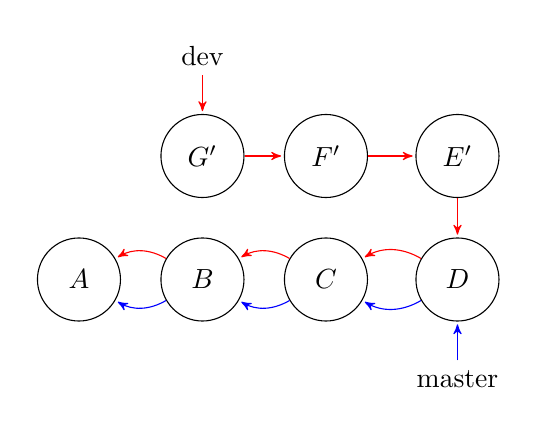
\begin{tikzpicture}[node distance=1.5cm]
            \matrix[row sep=5mm, column sep=5mm]{
                \& \node[branch] (dev) {dev} ; \& \& \\
                \&
                \node[commit] (G) {$G^\prime$} ; \&
                \node[commit] (F) {$F^\prime$} ; \&
                \node[commit] (E) {$E^\prime$} ; \\

                \node[commit] (A) {$A$} ; \&
                \node[commit] (B) {$B$} ; \&
                \node[commit] (C) {$C$} ; \&
                \node[commit] (D) {$D$} ; \\
                \& \& \& \node[branch] (master) {master} ; \\
            } ;

            \graph[use existing nodes]{
                master ->[branch']
                D ->[draw=blue,bend left]
                C ->[draw=blue,bend left]
                B ->[draw=blue,bend left]
                A ;

                dev ->[draw=red]
                G ->[draw=red]
                F ->[draw=red]
                E ->[draw=red]
                D ->[draw=red,bend right]
                C ->[draw=red,bend right]
                B ->[draw=red,bend right]
                A ;
            } ;
        \end{tikzpicture}
    \end{center}

    Arrows are duplicated only for clarity here, to show which commits belong
    to which branches.
\end{frame}

\begin{frame}
    \frametitle{Concept: the work tree}

    \begin{itemize}
        \item
            The \emph{work tree} is the directory that houses the code you work
            on.
            %
        \item
            Typically, the work tree contains the folder \texttt{.git} which
            houses the \emph{repository}.
            %
        \item
            Any directory can be made into the work tree of an empty repository
            by running \texttt{git init} in that directory.
            This is how a new project is started.
            %
        \item
            A special pointer called \HEAD{} serves as a reference point for
            what the working tree is supposed to be based on.
    \end{itemize}
\end{frame}

\begin{frame}
    \frametitle{Concept: the \HEAD{} pointer}

    \HEAD{} can be in one of two states, depending on what kind of thing it
    points to.

    \begin{description}
        \item[Attached:] \HEAD{} points to a branch.
        \item[Detached:] \HEAD{} points directly to a commit.
    \end{description}

    Whether \HEAD{} is attached or not affects the behaviour of several
    commands.

    In a newly initialized work tree and repository, \HEAD{} is attached to the
    \texttt{master} branch.
    (Even though this branch does not exist, as there are no commits in the
    repository yet!)
\end{frame}

\begin{frame}[fragile]
    \frametitle{Command-line: repository setup and creating commits}

    \begin{lstlisting}
mkdir -p projects/git-workshop
cd projects/git-workshop
git init
echo '# My awesome project' > README.md
git add README.md
git commit
    \end{lstlisting}

    Git will complain if it doesn't know your name and email since this
    information is recorded in the commit.

    \begin{lstlisting}
git config --global user.name "Linus Torvalds"
git config --global user.email "me@example.com"
    \end{lstlisting}
\end{frame}

\begin{frame}
    \frametitle{Command-line: \texttt{git add}}

    \begin{itemize}
        \item
            Using \texttt{git add} we specify which changes in our code should
            be included in the new commit.

            \protip{
                Use \texttt{git add -p} (short for \texttt{--patch}) to
                interactively add only portions of files that changed.
            }
            %
        \item
            These changes are recorded to a staging area called the
            \emph{index}.
            %
    \end{itemize}
\end{frame}

\begin{frame}
    \frametitle{Concept: committing}

    When \texttt{git commit} is invoked...

    \begin{itemize}
        \item
            The changes recorded in the index are applied to the snapshot of
            the commit pointed to by \HEAD{} to form a new snapshot.
            %
        \item
            Your name, email address, and the current time are added as
            metadata to the snapshot to form the new commit.
            %
        \item
            The parent of the new commit is the commit pointed to by \HEAD.
            %
        \item
            If \HEAD{} is attached to branch $X$, then $X$ advances to point to
            the new commit.
            %
        \item
            If \HEAD{} is detached, then \HEAD{} advances to point to the new
            commit.
            %
    \end{itemize}
\end{frame}

\begin{frame}
    \frametitle{Command-line: \texttt{git status}}

    \texttt{git status} indicates the current branch and describes the state of
    the work tree in three sections.

    \begin{itemize}
        \item \textit{Changes to be committed.}
            Describes the contents of the index.

        \item \textit{Changes not staged for commit.}
            Files that are present in the previous commit, identified by
            \HEAD, and have been modified.

        \item \textit{Untracked files.}
            Files that do not appear in the previous commit.
    \end{itemize}
\end{frame}

\begin{frame}
    \frametitle{Command-line: \texttt{git checkout}}

    \texttt{git checkout <branch>} switches branches.

    \begin{itemize}
        \item
            \HEAD{} is set to the given value.
            (This means you can checkout a commit directly too, making \HEAD{}
            detached.)
            %
        \item
            The contents of the identified commit is copied to the work tree.
            %
    \end{itemize}

    This command can be used also for copying specific files from a given
    commit into the current work tree.

    \protip{\texttt{git checkout --patch}}
\end{frame}

\begin{frame}
    \frametitle{Command-line: \texttt{git reset}}

    \texttt{git reset <commit>} makes the current branch, identified by
    \HEAD{}, point to a given commit. The way this command treats the index and
    work tree depends on which mode is used.

    \begin{description}
        \item[\texttt{--soft}]
            The index and work tree are unchanged.
            %
        \item[\texttt{--mixed}]
            The index is dropped, but the work tree is unchanged. (This mode is
            the default.)
            %
        \item[\texttt{--hard}]
            The index is dropped, and the contents of the commit is copied to
            the work tree, dropping and changes.
            %
    \end{description}

    If the given commit is itself \HEAD{}, then this command can be used to
    undo the action of \texttt{git add}.

    \protip{
        When a commit is unspecified in a command, it usually defaults to
        \HEAD{}.
    }

    \protip{
        \texttt{git reset --patch} can be used to interactively undo parts of a
        \texttt{git add}
    }
\end{frame}

\end{document}
